\documentclass[conference, 12pt]{IEEEtran}
\linespread{1.1}

\usepackage{graphicx}
\usepackage{cite}
\usepackage{amsmath}
\usepackage{amssymb}
\usepackage{lipsum}
\usepackage{microtype}
\setlength{\emergencystretch}{3em}
\tolerance=1000

\title{An Analysis on Testing Reliability Using Fault Injection }

\author{
    \IEEEauthorblockN{Vasileios Zoidis, Savvas Tzanetis}
    \IEEEauthorblockA{
        Department of Electrical and Computer Engineering\\
        Aristotle University of Thessaloniki
    }
}

\begin{document}

\maketitle

\begin{abstract}
Electronic systems, particularly space-borne applications, are increasingly vulnerable to temporary and permanent failures caused by environmental factors — most notably ionizing radiation. This vulnerability is becoming more pronounced as semiconductor feature sizes shrink and technologies scale. Consequently, the resilience of safety-critical aerospace and embedded platforms is compromised by faults such as Single Event Upsets (SEUs) and Multiple-Bit Upsets (MBUs). To mitigate these risks, systematic reliability assessment has become an essential component of system validation, necessitating the purposeful injection of errors to monitor system behavior.

This paper presents a comprehensive overview of fault injection as a reliability evaluation technique, tracing its evolution from historical origins to contemporary implementations. It examines modern fault injection methodologies across hardware, software, simulation and emulation domains, highlighting their ability to realistically reproduce radiation-induced faults and timing violations. Furthermore, representative case studies from the literature are analyzed to illustrate how fault injection validates fault tolerance mechanisms in embedded and flight software systems.

Overall, this work demonstrates that fault injection remains an indispensable tool for reliability engineering. While no single approach provides complete coverage, the combined use of hardware, software, simulation and emulation-based techniques enables comprehensive reliability assessment, supporting the design of resilient systems capable of operating in fault-prone environments.
\end{abstract}

% --- Introduction ---
\section{Introduction}
A common challenge in the design of semiconductor technologies is the sensitivity of electronics to cosmic radiation. This phenomenon is becoming increasingly apparent as technologies scale toward smaller feature sizes, altering the functionality of modern processors and FPGAs. This is particularly critical in safety domains such as automotive systems and space exploration, where even a single undetected error can lead to catastrophic failure, data corruption, or loss of mission objectives.

Specifically, ionizing radiation from cosmic rays can alter information stored in transistors. As a charged particle traverses a memory cell, it can deposit sufficient charge to invert a bit's logical state. This phenomenon is known as a \textit{bit-flip} error. Figure \ref{fig:radiation} illustrates this behavior.

\begin{figure}[htbp]
    \centering
    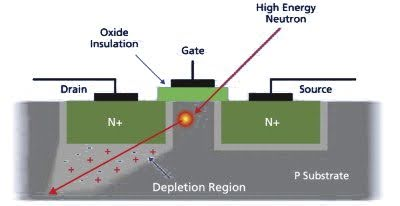
\includegraphics[width=1\linewidth]{assets/bitflip.jpg}
    \caption{Bit Altering Caused by Cosmic Rays}
    \label{fig:radiation}
\end{figure}

These faults fall into two categories, a \textit{Single Event Upset (SEU)}, where a single bit is altered in a device's memory, and \textit{Multiple-Bit Upsets (MBU)}, where several adjacent bits are corrupted simultaneously. \textit{MBUs} have become increasingly prevalent as technology is evolving and memory is becoming more dense.\\

Ensuring system reliability under such conditions requires more than theoretical fault models or post-deployment observation. Instead, engineers must proactively evaluate system behavior under similar fault conditions during the design and validation process. For this reason, fault injection has emerged as a key engineering methodology, by introducing actual faults into a system in order to observe and test its response, with the goal of designing fault tolerance mechanisms.\\

Fault Injection approaches can be broadly classified into three categories:
\begin{enumerate}
    \item \textbf{Hardware-based techniques:} Using physical equipment (e.g., radiation sources or pin injection) to alter device states.
    \item \textbf{Software-Implemented Fault Injection (SWIFI):} Using software routines to corrupt memory or registers at the operating system or application level.
    \item \textbf{Simulation and Emulation:} Utilizing Instruction Set Architecture (ISA) simulators or Register Transfer Level (RTL) models to inject faults into virtual hardware descriptions, enabling early analysis of both reliability and resource utilization without physical prototypes.
\end{enumerate}

% --- Historical Overview ---
\section{Historical Overview}

\subsection{Early Physical Fault Injection}
The earliest fault injection efforts were closely tied to the study of radiation effects on electronic systems, driven primarily by organizations such as IBM and NASA in the 1970s. During this period, reliability concerns were motivated by space exploration and high-altitude avionics, where radiation exposure is significantly higher than at ground level.\\

Initial techniques relied on direct physical fault injection by attempting to reproduce the effects of radiation-induced disturbances using particle accelerators. Such accelerators were capable of inducing heavy-ion and neutron irradiation to electronic components, causing SEUs. While this approach provided high physical fidelity, it was expensive, time consuming, and limited to specialized facilities.\\

Another early approach was direct fault injections by manipulating the voltage and amperage in the pins of a processor, resulting in the unexpected tweaking of signal timings and causing transient or permanent faults. As can be imagined though, this technique became obsolete as integrated circuits became more complex and pin counts both increased while their size decreased, ultimately becoming impossible to tweak. Furthermore, deeply embedded transistors and internal interconnects were no longer directly accessible from package pins.

\subsection{Transition to Software-Implemented Fault Injection}
After the physical constraints that appeared in the early days of fault injection, in the late 1980s and early 1990s, the research community focused on other methods for causing fault injection, where the emergence of software implemented fault injection (SWIFI) techniques began. This technique relied on manipulating a system's state through software mechanisms running on the system hardware itself.\\

Seminal tools such as \textit{FIAT} (1990) \cite{FIAT} and \textit{FERRARI} (1992) \cite{FERRARI} introduced controlled corruption of memory locations, registers, and variables during program execution. In general, a typical SWIFI workflow involves temporarily halting program execution, flipping one or more bits at a selected memory address, and resuming execution to observe the resulting behavior. This approach effectively simulates SEUs without requiring specialized hardware or radiation facilities.\\

Using software techniques significantly reduced the cost and time of creating tests, and increased experimental flexibility. However, it also introduced abstraction limitations, as not all hardware level faults such as timing violations or power transients were able to be reproduced.

\subsection{Pre-Silicon Simulation and Emulation-Based Injection}
Lastly, as system complexity increased, the validation of a system's reliability shifted to earlier stages of design and fabrication. Simulation and emulation based fault injection techniques arose, operating on hardware description language (HDL) models of digital systems before physical manufacturing.\\

Tools such as \textit{MEFISTO} \cite{MEFISTO} enable designers to test fault tolerance in digital systems by intentionally inserting faults into the hardware description language model during simulation. Faults may include bit flips in registers, corrupted signals in interconnects, or timing delays in combinational logic. This virtual environment grants comprehensive control over the system's state, allowing for precise fault injection and observation of the resulting error propagation through the simulated architecture.\\

While simulation based methods are significantly faster and cheaper than physical testing, they rely on the accuracy of the underlying models. Missing architectural details or unmodeled hardware exceptions can lead to discrepancies between simulated behavior and real hardware responses.

% ----- Hardware -----
\section{Fault Injection using Hardware Tools}
Returning to hardware-based fault injection techniques, these days researchers may use several methods for introducing faults to a system. One such methodology uses EMP (Electromagnetic Pulse) devices to generate pulses strong enough to interfere with the logic of modern electronics. An example of such a device can be seen in Figure \ref{fig:emp_device}. \\

\begin{figure}[htbp]
    \centering
    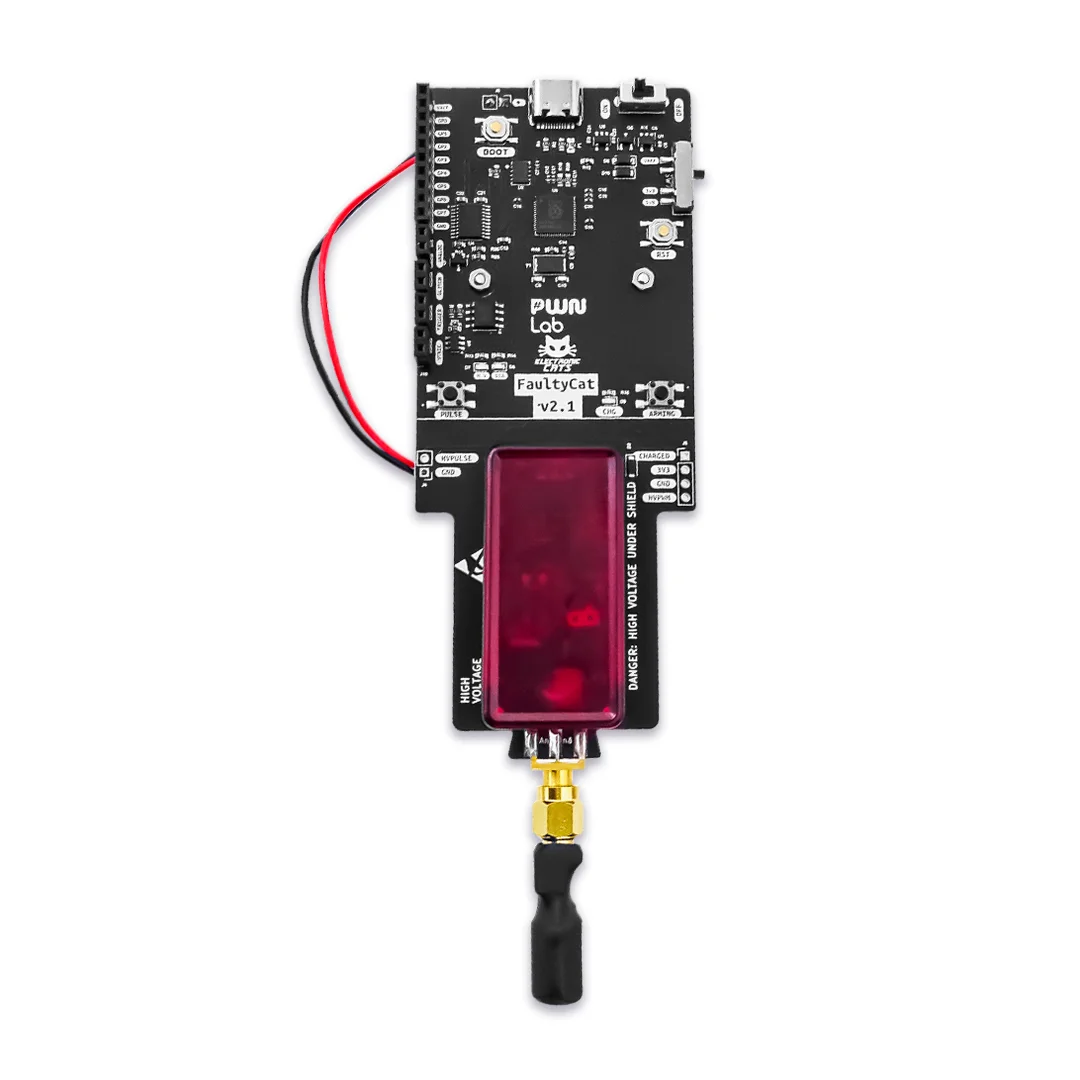
\includegraphics[width=0.5\linewidth]{assets/faultycat.png}
    \caption{EM Fault Injection Device}
    \label{fig:emp_device}
\end{figure}

Another hardware-based fault injection method utilizes the broad capabilities of an FPGA system, especially programmed to disrupt the signals of the components that manufacturers want to test, by being connected to them. These sub-systems are capable of modifying memory addresses in a program as well as cause pseudo-randomized bit-flips. Using FPGAs, researchers are capable of producing both SEUs and MBUs, as well as cause clock glitches, or even power glitches, all of which are broadly observed in areas such as space exploration or aviation. \\

These techniques can be applied in both conventional Von-Neumann processors like the ones commonly found in smartphones, as well as other FPGAs systems. In the case of fault injection in FPGA systems, it is also possible to reserve a portion of the system's maximum utilization for injecting faults, as previously discussed.

\subsection{Hardware Fault Injection using FISH}
Focusing in more detail on hardware-based fault injection using FPGAs, \textit{FISH} (Fault Injection Self-test Hardware) is a method proposed by Shandilya, Rahul, and Sharma, R.\cite{HardwareSite} and aims to create self-testing hardware, able to effectively inject MBU faults into the rest of the system. The proposed implementation consists of 4 8-bit LFSRs (Linear Feedback Shift Registers) that are tasked with creating a pseudo-randomized string of numbers that will determine which bits in the memory are flipped during the fault injection process. A programmable LFSR circuit can be viewed in Figure \ref{fig:lfsr}. \\

\begin{figure}[htpb]
    \centering
    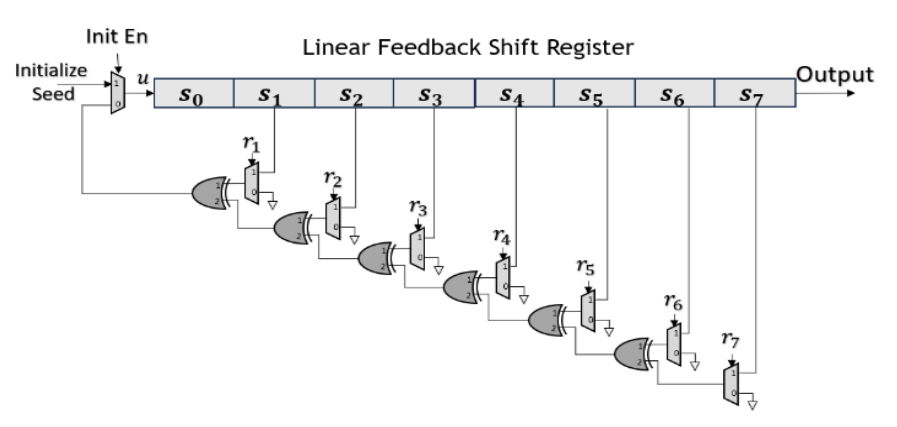
\includegraphics[width=0.9\linewidth]{assets/lfsr_circuit.png}
    \caption{Programmable LFSR Circuit}
    \label{fig:lfsr}
\end{figure}

As stated in the paper, the LFSRs functions by initially using a seed as a base number sequence, and shifting its values while using the previous outputs of the register as new inputs to determine how much a number is going to be shifted, generating whitening sequences,
pseudo-noise sequences, pseudo-random numbers, etc. \\

The complete circuit of the fault injection sub-system is composed of the four previously mentioned LFSRs, in addition to hardware logic responsible for control and programming, and can be viewed in Figure \ref{fig:complete_fish}. Additionally, the fault injection input sequence that feeds in the design can be read-back from Serial in Parallel Out (SIPO). The captured data is later evaluated on the basis of number of ones and used for classification of faults that were generated during the whole process.

\begin{figure}[htbp]
    \centering
    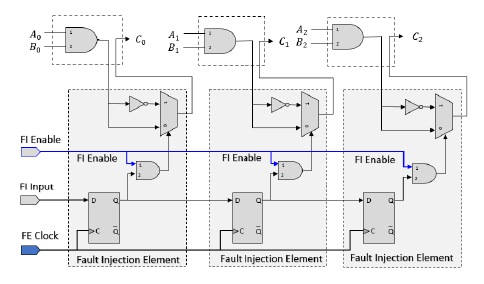
\includegraphics[width=0.9\linewidth]{assets/fish.png}
    \caption{Complete FISH Logic Circuit}
    \label{fig:complete_fish}
\end{figure}

The methodology proposed by Shandilya, Rahul and Sharma, R. demonstrates notably improved performance when compared to \textit{BUFIT} and \textit{SCFIT}, both of which are hardware-based fault injection techniques commonly used for reliability evaluation. \textit{BUFIT} primarily focuses on single-bit fault injection through direct modification of flip-flop states, offering simplicity, while lacking support for realistic multi-bit upset scenarios. On the other hand, \textit{SCFIT} introduces faults by targeting scan-chain elements, enabling structured fault insertion but at the cost of increased design intrusion and reduced flexibility. 


As illustrated in Figure \ref{fig:results_fish}, FISH achieves a significantly higher fault injection rate of \texttt{111.1 faults/s} compared to the rest of the injection methods tested.

\begin{figure}[htbp]
    \centering
    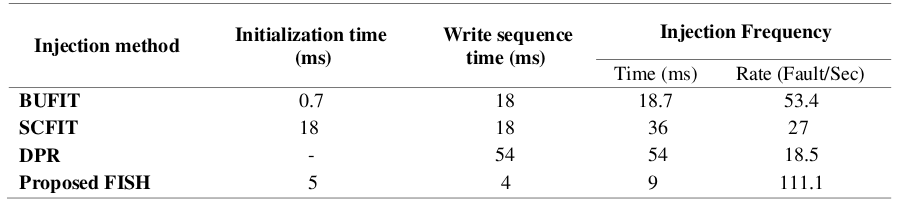
\includegraphics[width=0.9\linewidth]{assets/results_fish.png}
    \caption{Fault Injection Rate Comparison Between Techniques}
    \label{fig:results_fish}
\end{figure}

While the significantly higher injection rate of the proposed methodology plays an important factor in its usability, a more important role to consider is the hardware overhead needed for these implementations to function properly. As seen in Figure \ref{fig:fish_util}, which compares the utilization overhead of CLBs (Configurable Logic Blocks) and FFs (Flip Flops) of an FPGA programmed as an \textit{OR1200}, \textit{FISH} manages to stay relatively low in its usage requirements, comparing closely to the \textit{SCFIT} technique, which requires an extra 6\% of CLBs and 5.8\% of FFs to be added in addition to the FPGA target, while \textit{BUFIT}, shows a significantly less utilization overhead which is expected given its simplicity and lack of configurability. \\

\begin{figure}[htbp]
    \centering
    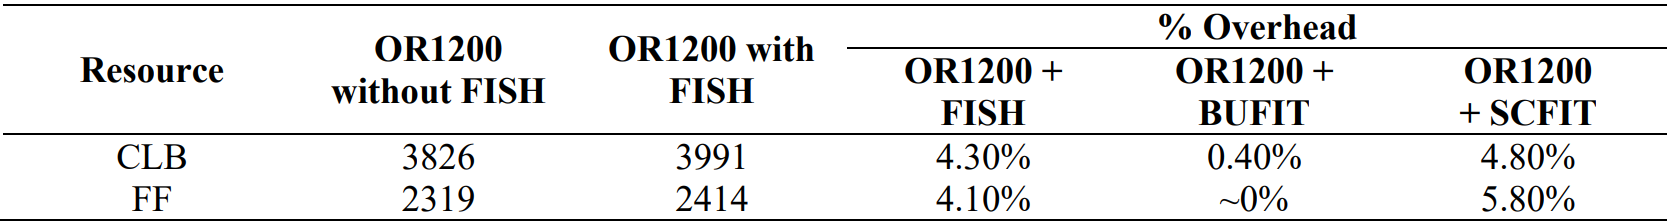
\includegraphics[width=0.9\linewidth]{assets/fish_util.png}
    \caption{Comparison of the Utilization of FI Techniques}
    \label{fig:fish_util}
\end{figure}

Overall, the experimental results indicate that FISH provides a more scalable and less intrusive solution for multi-bit fault injection, making it particularly suitable for reliability assessment of modern embedded and FPGA-based systems.

% ----- Software -----
\section{Fault Injection using Software Tools}

Software-Implemented Fault Injection (SWIFI) has become a prominent technique for evaluating system reliability, particularly as hardware complexity increases and physical access to internal components becomes more difficult. Unlike hardware-based methods that require physical probes or radiation sources, SWIFI emulates hardware faults by modifying software states, memory contents, or register values during program execution.

\subsection{Overview of SWIFI Techniques}
SWIFI techniques are generally classified into two main categories: compile-time and runtime injection. Compile-time injection involves modifying the source code or assembly code to insert fault triggers before the program is built. Runtime injection, which is largely more common, uses mechanisms such as interrupts, debuggers, or exception handlers to intercept program execution and alter the state of the processor or memory.

Common targets for SWIFI include:
\begin{itemize}
    \item \textbf{CPU Registers:} Corrupting general-purpose or special-purpose registers to simulate transient CPU faults.
    \item \textbf{Memory:} Flipping bits in  text code, data, heap, or stack segments to emulate Single Event Upsets (SEUs) in RAM.
    \item \textbf{I/O Interfaces:} Intercepting and corrupting data packets to test communication protocols.
\end{itemize}

SWIFI is highly valued for its low cost, flexibility, and ability to target specific software structures. However, it suffers from intrusiveness, as the injection code itself adds overhead, potentially missing real-world timing issues, making it less useful for sensitive real-time systems.

\subsection{Case Study: Failure Assessment of NASA cFS Case-Study Flight Software on RISC-V via Fault Injection}
A recent study by Fran\c{c}a et al. \cite{SoftwareSite} demonstrates the application of SWIFI to assess the reliability of safety-critical flight software. This case study evaluates NASA's Core Flight System (cFS), a reusable software framework used in missions like the Lunar Reconnaissance Orbiter and the James Webb Space Telescope, running on a RISC-V PolarFire System-on-Chip (SoC).

The study utilized a fault injection campaign to simulate radiation-induced faults in Low Earth Orbit (LEO). The experimental setup involved a RISC-V PolarFire SoC running the FreeRTOS operating system with a port of NASA's Operating System Abstraction Layer (OSAL). Faults were injected into the volatile memory (RAM) where application data, stack, and heap were stored. A Python-based host script communicated with the target via a serial port interrupt to trigger bit-flips at random memory addresses and time intervals. As the workload, two benchmark applications were used as probes: Huffman encoding/decoding and Fixed-Point Matrix Multiplication.

\begin{figure}[htbp]
    \centering
    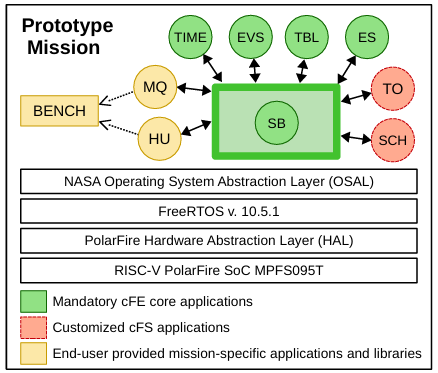
\includegraphics[width=0.75\linewidth]{assets/Mission software stack.png}
    \caption{Mission software stack}
    \label{fig:Mission}
\end{figure}

The campaign observed 2,270 functional failures, classifying them into three categories: I/O Timeouts (system hang), Silent Data Corruption (SDC) and Result Timeouts. Approximately 79\% of the observed failures resulted in the flight software becoming unresponsive (I/O Timeout), requiring a hardware reset. The system remained active but produced incorrect results 12\% of the time (SDC) and it transmitted data that could not be decoded 9\% of the time
(Result Timeout).

By utilizing FreeRTOS trace resources, the study identified that the cFS Scheduler (SCH) task was the most sensitive to faults. Failures during the SCH task execution accounted for over 21\% of the total failures. The study mapped failure rates to specific memory footprints. For instance, the Event Services (EVS) task, despite having a small footprint, showed a disproportionately high number of failures, indicating high architectural vulnerability.

\begin{figure}[htbp]
    \centering
    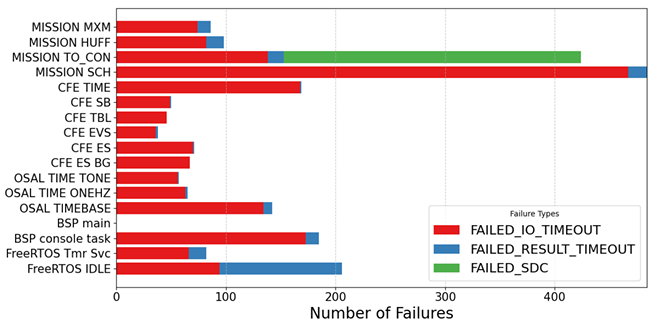
\includegraphics[width=0.9\linewidth]{assets/SWIFI_failures.png}
    \caption{Number of Failures detected while the task was executing.}
    \label{fig:SWIFI_failures}
\end{figure}

This case study illustrates how SWIFI can effectively identify critical software modules (e.g., the Scheduler) that require hardening, enabling targeted fault tolerance improvements without the need for expensive radiation testing facilities. Furthermore, it demonstrated the viability of NASA's cFS framework on open source platforms such as RISC-V and FreeRTOS.

% --- Emulation/Simulation ---
\section{Fault Injection using Emulation and Simulation Tools}

While Software-Implemented Fault Injection is effective for assessing software resilience, it is often limited by its inability to access low-level hardware states (such as pipeline registers) or accurately model timing-dependent hardware behaviors. Conversely, physical hardware injection offers ultimate realism but lacks observability and is often prohibitively expensive. Emulation and simulation-based fault injection serve as a crucial middle ground, bridging this gap by utilizing models to inject hardware-level faults while maintaining the high controllability and visibility typical of software approaches.

\subsection{Simulation vs. Emulation}
Simulation-based injection typically uses Instruction Set Architecture (ISA) simulators or Register Transfer Level (RTL) models. It offers high controllability and visibility, allowing injection into any architectural state (e.g., hidden pipeline registers). However, it often trades execution speed for accuracy and is bound by the model limitations, where it cannot simulate certain hardware features such as timers and exceptions.

On the other hand, emulation-based injection is highly accurate as it is able to record the real behavior of the device.
However, while gaining in accuracy it lacks in speed and as a result emulation campaigns often last hours. Moreover, this performance comes at the cost of visibility; unlike simulation, emulation is limited to the resources exposed by the hardware interface, often leaving internal micro-architectural structures (such as pipeline registers) inaccessible for injection or monitoring.

\subsection{Case Study: Evaluation of fault injection tools for reliability estimation of microprocessor-based embedded systems}
A study by Aponte-Moreno et al. \cite{EmulationSite} presents a rigorous quantitative comparison between simulation and emulation tools. The researchers evaluated the reliability of a Texas Instruments MSP430 microcontroller using three distinct tools:
\begin{itemize}
    \item \textbf{MiFIT:} A modular, open-source ISA simulator.
    \item \textbf{Naken-FIM:} A modified instruction-accurate simulator with enhanced trace capabilities.
    \item \textbf{FIM:} An emulation-based framework utilizing the On-Chip Debugging (OCD) infrastructure of the physical MSP430 device.
\end{itemize}

The study injected bit-flips into the register file and memory sections (.data, .stack, .text) while running standard benchmarks (Euler, QuickSort, Matrix Multiplication) per clock cycle or per instruction, in the case of simulators (Figure \ref{fig:Percentage}). The results were compared against ground-truth data from neutron beam irradiation experiments at the Los Alamos Neutron Science Center (LANSCE).

\begin{figure}[htbp]
    \centering
    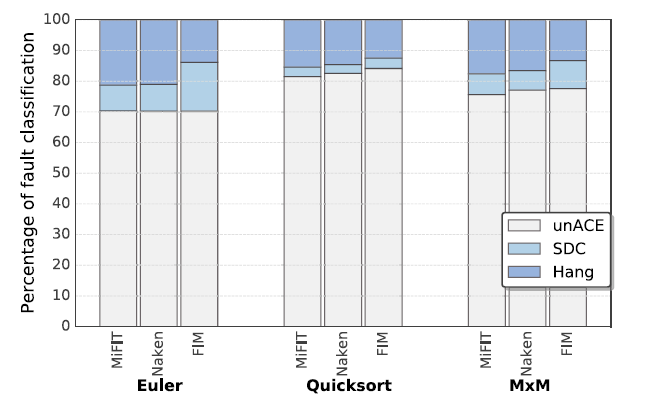
\includegraphics[width=0.9\linewidth]{assets/Percentage of fault classification.png}
    \caption{Percentage of fault classification for each benchmark.}
    \label{fig:Percentage}
\end{figure}

The comparison revealed that while simulation tools are faster, they can overestimate certain failure modes.

At first, the simulation tools (MiFIT and Naken) showed consistent results with each other, with differences in fault classification (e.g., Silent Data Corruption vs. Hang) of less than 3.3\% for the register file. However, they were significantly off from the emulation tool's results, and gave a reliability estimate that was 10\% lower.

More specifically, significant deviations were observed in critical registers such as the Program Counter (R0), the Stack Pointer (R1) and other non-critical registers depending on the benchmark application (Figure \ref{fig:Registers}). These differences were mainly due to the limitations of the simulator models; For example, in the Euler benchmark, faults in register R6 caused a "Hang" in the simulator but a "Silent Data Corruption" (SDC) in the emulator. This difference was attributed to the simulators' simplified handling of execution time. The researchers observed that the real hardware continued executing "trash code" longer than the simulator allowed, thus, misclassifying the fault for only a few cycles of discrepancy. Extending the simulator's timeout limit significantly reduced this gap.

\begin{figure}[htbp]
    \centering
    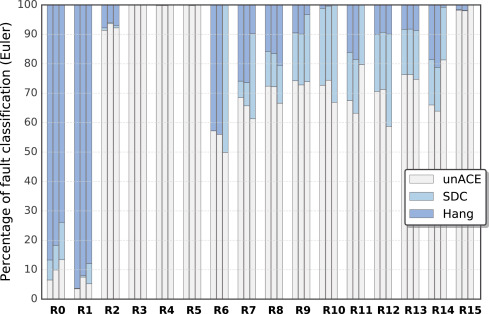
\includegraphics[width=0.9\linewidth]{assets/register-faults.jpg}
    \caption{Percentages of fault classification in the register file by fault injection tool (MiFIT, Naken, and FIM) for Euler}
    \label{fig:Registers}
\end{figure}

Furthermore, simulation tools often lacked accurate models for hardware exceptions. Faults injected into the stack pointer (SP) on the real device often triggered system resets or traps, that the ISA simulators processed as valid jumps to uninitialized memory. This also led to divergent failure classifications.

Overall, the study concludes that ISA-level simulation is highly effective for preliminary design space exploration, offering a speed advantage for tuning fault mitigation techniques. However, for final validation, emulation or hybrid approaches are necessary to capture micro-architectural behaviors (such as pipeline stalls and hardware exceptions) that simulators often abstract away.

\subsection{Case Study: RTL-Based Reliability and Resource Analysis of Spaceborne FPGAs}
While ISA-level simulation focuses on software behavior, simulation at the Register Transfer Level (RTL) enables the evaluation of hardware fault tolerance mechanisms (FTMs) early in the design phase. A 2025 study by Kim et al. \cite{AerospaceSiteEmu} utilized this approach to analyze the trade-offs between reliability and resource utilization in spaceborne electronic systems.

The study targeted an AES-128 encryption circuit, a critical component for secure space communications. To assess reliability, the authors employed Statistical Fault Injection (SFI) using the \textit{Verilog Fault Injector} on the \textit{Icarus Verilog} simulator. They injected single-bit and multi-bit faults (reflecting Single Event Upsets) into the circuit's key expansion and round modules.

Unlike the software-focused metrics of ISA simulators, this RTL-based approach allowed for the calculation of the \textit{Architectural Vulnerability Factor} (AVF) alongside physical resource metrics defined as the Power-Delay-Area Product (PDAP):
\begin{equation}
    PDAP = Power \times Delay \times Area
\end{equation}
This metric provided a quantitative basis for comparing hardware redundancy (e.g., TMR) against information redundancy (e.g., Hamming Code)(Figure \ref{fig:Classification}).

\begin{figure} [htbp]
    \centering
    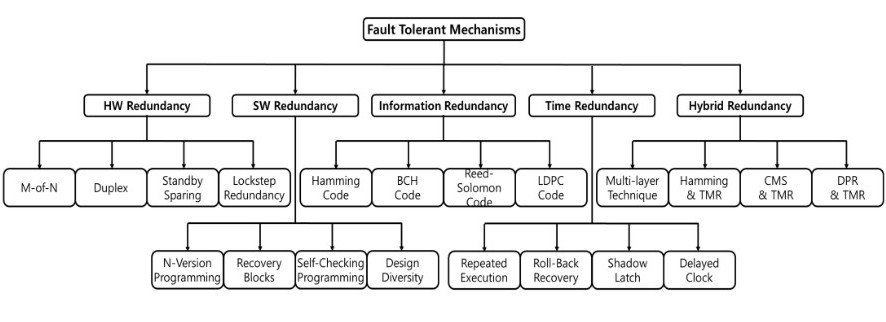
\includegraphics[width=0.9\linewidth] {assets/classification.jpg}
    \caption{Classification of fault-tolerant mechanisms for electronic equipment}
    \label{fig:Classification}
\end{figure}

The simulation results highlighted distinct trade-offs between the two redundancy categories:

\begin{itemize}
    \item \textbf{Information Redundancy:} The Hamming Code mechanism achieved high reliability, reducing the AVF significantly. However, it incurred a massive resource penalty, increasing the PDAP by approximately 355\% compared to the baseline due to the complexity of encoding/decoding logic.
    \item \textbf{Hardware Redundancy:} Triple Modular Redundancy (TMR) offered the most efficient balance. While its reliability was slightly lower than the most robust hybrid methods, it maintained a low resource overhead (PDAP), making it highly suitable for resource-constrained FPGA environments.
    \item \textbf{Hybrid Approaches:} A combined "Hamming \& TMR" mechanism yielded the highest reliability ($95.82\%$ fault masking) but at a prohibitive resource cost, with a PDAP increase of over 587\% (Figure \ref{fig:PDAP}).
\end{itemize}

\begin{figure} [htbp]
    \centering
    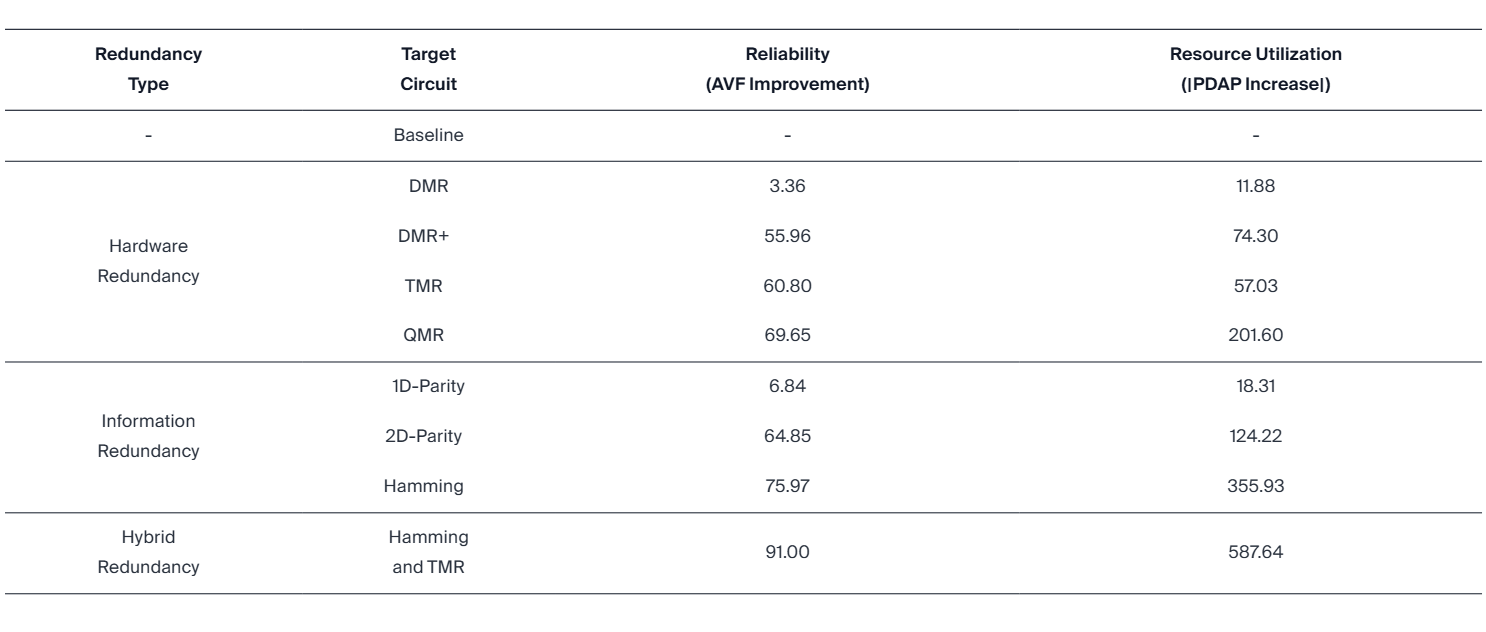
\includegraphics[width=0.9\linewidth] {assets/PDAP.png}
    \caption{Reliability and resource utilization analysis per target circuit}
    \label{fig:PDAP}
\end{figure}

This case study demonstrates that RTL simulation bridges the gap between high-level functional verification and physical implementation. It allows engineers to optimize the "Reliability vs. Resource" cost function before committing to silicon, a capability that neither pure software injection (SWIFI) nor physical emulation can easily provide.

% --- Conclusion ---
\section{Discussion \& Conclusion}
As semiconductor technology scales, the susceptibility of mission-critical systems to transient faults necessitates a rigorous and multi-faceted reliability assessment. This work has analyzed the different techniques for achieving Fault Injection, demonstrating that no single approach can provide complete results. Alternatively, they serve complementary roles across the system design's life cycle.

Hardware-based techniques remain superior for replicating complex physical phenomena, such as Multiple-Bit Upsets (MBUs), with high fidelity. However, as systems grow in complexity, the abstraction provided by Software-Implemented Fault Injection (SWIFI) becomes crucial. The analysis of NASA’s Core Flight System highlighted SWIFI's efficacy in pinpointing application level vulnerabilities, identifying a system's scheduler as a critical failure point without requiring specialized physical setups.

Crucially, this paper also examined the role of Simulation and Emulation in bridging the gap between software logic and physical implementation. While Instruction Set Architecture (ISA) simulators allow for rapid software tuning, they often lack the micro architectural fidelity to model hardware exceptions accurately, potentially underestimating reliability metrics by up to 10\% compared to physical emulation.

Conversely, Register Transfer Level (RTL) simulation has proven indispensable for early hardware optimization. As demonstrated by the analysis of spaceborne FPGAs, RTL-based injection enables the quantification of the \textit{Power-Delay-Area Product (PDAP)}.

Ultimately, comprehensive reliability engineering requires a hybrid strategy:
\begin{itemize}
    \item \textbf{RTL Simulation} for early "reliability vs. resource" trade-off analysis and sizing of fault tolerance mechanisms.
    \item \textbf{SWIFI} for verifying software logic, task isolation, and error recovery routines.
    \item \textbf{Hardware Emulation} for final validation where micro-architectural timing and exception handling are paramount.
\end{itemize}
By integrating these diverse methodologies, engineers can ensure the design of resilient systems capable of robust operation in harsh, fault prone environments.

% --- Bibliography ---
\bibliographystyle{IEEEtran}
\bibliography{references}

\end{document}
